\documentclass{ximera}  

%\usepackage{todonotes}
%\usepackage{mathtools} %% Required for wide table Curl and Greens
%\usepackage{cuted} %% Required for wide table Curl and Greens
\newcommand{\todo}{}

\usepackage{esint} % for \oiint
\ifxake%%https://math.meta.stackexchange.com/questions/9973/how-do-you-render-a-closed-surface-double-integral
\renewcommand{\oiint}{{\large\bigcirc}\kern-1.56em\iint}
\fi


\graphicspath{
  {./}
  {jpg}
  {ximeraTutorial/}
  {basicPhilosophy/}
  {functionsOfSeveralVariables/}
  {normalVectors/}
  {lagrangeMultipliers/}
  {vectorFields/}
  {greensTheorem/}
  {shapeOfThingsToCome/}
  {dotProducts/}
  {partialDerivativesAndTheGradientVector/}
  {../productAndQuotientRules/exercises/}
  {../motionAndPathsInSpace/exercises/}
  {../normalVectors/exercisesParametricPlots/}
  {../continuityOfFunctionsOfSeveralVariables/exercises/}
  {../partialDerivativesAndTheGradientVector/exercises/}
  {../directionalDerivativeAndChainRule/exercises/}
  {../commonCoordinates/exercisesCylindricalCoordinates/}
  {../commonCoordinates/exercisesSphericalCoordinates/}
  {../greensTheorem/exercisesCurlAndLineIntegrals/}
  {../greensTheorem/exercisesDivergenceAndLineIntegrals/}
  {../shapeOfThingsToCome/exercisesDivergenceTheorem/}
  {../greensTheorem/}
  {../shapeOfThingsToCome/}
  {../separableDifferentialEquations/exercises/}
  {vectorFields/}
}

\newcommand{\mooculus}{\textsf{\textbf{MOOC}\textnormal{\textsf{ULUS}}}}

\usepackage{tkz-euclide}\usepackage{tikz}
\usepackage{tikz-cd}
\usetikzlibrary{arrows}
\tikzset{>=stealth,commutative diagrams/.cd,
  arrow style=tikz,diagrams={>=stealth}} %% cool arrow head
\tikzset{shorten <>/.style={ shorten >=#1, shorten <=#1 } } %% allows shorter vectors

\usetikzlibrary{backgrounds} %% for boxes around graphs
\usetikzlibrary{shapes,positioning}  %% Clouds and stars
\usetikzlibrary{matrix} %% for matrix
\usepgfplotslibrary{polar} %% for polar plots
\usepgfplotslibrary{fillbetween} %% to shade area between curves in TikZ
\usetkzobj{all}
\usepackage[makeroom]{cancel} %% for strike outs
%\usepackage{mathtools} %% for pretty underbrace % Breaks Ximera
%\usepackage{multicol}
\usepackage{pgffor} %% required for integral for loops



%% http://tex.stackexchange.com/questions/66490/drawing-a-tikz-arc-specifying-the-center
%% Draws beach ball
\tikzset{pics/carc/.style args={#1:#2:#3}{code={\draw[pic actions] (#1:#3) arc(#1:#2:#3);}}}



\usepackage{array}
\setlength{\extrarowheight}{+.1cm}
\newdimen\digitwidth
\settowidth\digitwidth{9}
\def\divrule#1#2{
\noalign{\moveright#1\digitwidth
\vbox{\hrule width#2\digitwidth}}}





\newcommand{\RR}{\mathbb R}
\newcommand{\R}{\mathbb R}
\newcommand{\N}{\mathbb N}
\newcommand{\Z}{\mathbb Z}

\newcommand{\sagemath}{\textsf{SageMath}}


%\renewcommand{\d}{\,d\!}
\renewcommand{\d}{\mathop{}\!d}
\newcommand{\dd}[2][]{\frac{\d #1}{\d #2}}
\newcommand{\pp}[2][]{\frac{\partial #1}{\partial #2}}
\renewcommand{\l}{\ell}
\newcommand{\ddx}{\frac{d}{\d x}}

\newcommand{\zeroOverZero}{\ensuremath{\boldsymbol{\tfrac{0}{0}}}}
\newcommand{\inftyOverInfty}{\ensuremath{\boldsymbol{\tfrac{\infty}{\infty}}}}
\newcommand{\zeroOverInfty}{\ensuremath{\boldsymbol{\tfrac{0}{\infty}}}}
\newcommand{\zeroTimesInfty}{\ensuremath{\small\boldsymbol{0\cdot \infty}}}
\newcommand{\inftyMinusInfty}{\ensuremath{\small\boldsymbol{\infty - \infty}}}
\newcommand{\oneToInfty}{\ensuremath{\boldsymbol{1^\infty}}}
\newcommand{\zeroToZero}{\ensuremath{\boldsymbol{0^0}}}
\newcommand{\inftyToZero}{\ensuremath{\boldsymbol{\infty^0}}}



\newcommand{\numOverZero}{\ensuremath{\boldsymbol{\tfrac{\#}{0}}}}
\newcommand{\dfn}{\textbf}
%\newcommand{\unit}{\,\mathrm}
\newcommand{\unit}{\mathop{}\!\mathrm}
\newcommand{\eval}[1]{\bigg[ #1 \bigg]}
\newcommand{\seq}[1]{\left( #1 \right)}
\renewcommand{\epsilon}{\varepsilon}
\renewcommand{\phi}{\varphi}


\renewcommand{\iff}{\Leftrightarrow}

\DeclareMathOperator{\arccot}{arccot}
\DeclareMathOperator{\arcsec}{arcsec}
\DeclareMathOperator{\arccsc}{arccsc}
\DeclareMathOperator{\si}{Si}
\DeclareMathOperator{\scal}{scal}
\DeclareMathOperator{\sign}{sign}


%% \newcommand{\tightoverset}[2]{% for arrow vec
%%   \mathop{#2}\limits^{\vbox to -.5ex{\kern-0.75ex\hbox{$#1$}\vss}}}
\newcommand{\arrowvec}[1]{{\overset{\rightharpoonup}{#1}}}
%\renewcommand{\vec}[1]{\arrowvec{\mathbf{#1}}}
\renewcommand{\vec}[1]{{\overset{\boldsymbol{\rightharpoonup}}{\mathbf{#1}}}\hspace{0in}}

\newcommand{\point}[1]{\left(#1\right)} %this allows \vector{ to be changed to \vector{ with a quick find and replace
\newcommand{\pt}[1]{\mathbf{#1}} %this allows \vec{ to be changed to \vec{ with a quick find and replace
\newcommand{\Lim}[2]{\lim_{\point{#1} \to \point{#2}}} %Bart, I changed this to point since I want to use it.  It runs through both of the exercise and exerciseE files in limits section, which is why it was in each document to start with.

\DeclareMathOperator{\proj}{\mathbf{proj}}
\newcommand{\veci}{{\boldsymbol{\hat{\imath}}}}
\newcommand{\vecj}{{\boldsymbol{\hat{\jmath}}}}
\newcommand{\veck}{{\boldsymbol{\hat{k}}}}
\newcommand{\vecl}{\vec{\boldsymbol{\l}}}
\newcommand{\uvec}[1]{\mathbf{\hat{#1}}}
\newcommand{\utan}{\mathbf{\hat{t}}}
\newcommand{\unormal}{\mathbf{\hat{n}}}
\newcommand{\ubinormal}{\mathbf{\hat{b}}}

\newcommand{\dotp}{\bullet}
\newcommand{\cross}{\boldsymbol\times}
\newcommand{\grad}{\boldsymbol\nabla}
\newcommand{\divergence}{\grad\dotp}
\newcommand{\curl}{\grad\cross}
%\DeclareMathOperator{\divergence}{divergence}
%\DeclareMathOperator{\curl}[1]{\grad\cross #1}
\newcommand{\lto}{\mathop{\longrightarrow\,}\limits}

\renewcommand{\bar}{\overline}

\colorlet{textColor}{black}
\colorlet{background}{white}
\colorlet{penColor}{blue!50!black} % Color of a curve in a plot
\colorlet{penColor2}{red!50!black}% Color of a curve in a plot
\colorlet{penColor3}{red!50!blue} % Color of a curve in a plot
\colorlet{penColor4}{green!50!black} % Color of a curve in a plot
\colorlet{penColor5}{orange!80!black} % Color of a curve in a plot
\colorlet{penColor6}{yellow!70!black} % Color of a curve in a plot
\colorlet{fill1}{penColor!20} % Color of fill in a plot
\colorlet{fill2}{penColor2!20} % Color of fill in a plot
\colorlet{fillp}{fill1} % Color of positive area
\colorlet{filln}{penColor2!20} % Color of negative area
\colorlet{fill3}{penColor3!20} % Fill
\colorlet{fill4}{penColor4!20} % Fill
\colorlet{fill5}{penColor5!20} % Fill
\colorlet{gridColor}{gray!50} % Color of grid in a plot

\newcommand{\surfaceColor}{violet}
\newcommand{\surfaceColorTwo}{redyellow}
\newcommand{\sliceColor}{greenyellow}




\pgfmathdeclarefunction{gauss}{2}{% gives gaussian
  \pgfmathparse{1/(#2*sqrt(2*pi))*exp(-((x-#1)^2)/(2*#2^2))}%
}


%%%%%%%%%%%%%
%% Vectors
%%%%%%%%%%%%%

%% Simple horiz vectors
\renewcommand{\vector}[1]{\left\langle #1\right\rangle}


%% %% Complex Horiz Vectors with angle brackets
%% \makeatletter
%% \renewcommand{\vector}[2][ , ]{\left\langle%
%%   \def\nextitem{\def\nextitem{#1}}%
%%   \@for \el:=#2\do{\nextitem\el}\right\rangle%
%% }
%% \makeatother

%% %% Vertical Vectors
%% \def\vector#1{\begin{bmatrix}\vecListA#1,,\end{bmatrix}}
%% \def\vecListA#1,{\if,#1,\else #1\cr \expandafter \vecListA \fi}

%%%%%%%%%%%%%
%% End of vectors
%%%%%%%%%%%%%

%\newcommand{\fullwidth}{}
%\newcommand{\normalwidth}{}



%% makes a snazzy t-chart for evaluating functions
%\newenvironment{tchart}{\rowcolors{2}{}{background!90!textColor}\array}{\endarray}

%%This is to help with formatting on future title pages.
\newenvironment{sectionOutcomes}{}{}



%% Flowchart stuff
%\tikzstyle{startstop} = [rectangle, rounded corners, minimum width=3cm, minimum height=1cm,text centered, draw=black]
%\tikzstyle{question} = [rectangle, minimum width=3cm, minimum height=1cm, text centered, draw=black]
%\tikzstyle{decision} = [trapezium, trapezium left angle=70, trapezium right angle=110, minimum width=3cm, minimum height=1cm, text centered, draw=black]
%\tikzstyle{question} = [rectangle, rounded corners, minimum width=3cm, minimum height=1cm,text centered, draw=black]
%\tikzstyle{process} = [rectangle, minimum width=3cm, minimum height=1cm, text centered, draw=black]
%\tikzstyle{decision} = [trapezium, trapezium left angle=70, trapezium right angle=110, minimum width=3cm, minimum height=1cm, text centered, draw=black]


\title{Sinusoidal Signals}  
\author{Milica Markovic}
\outcome{Recognize the basic properties of sinusoidal functions and relate them to circuit analysis.}
\begin{document}  
\begin{abstract}  
Review of Sinusoidal Signals
\end{abstract}  
\maketitle

\section{Sinusoidal signal parameters}

Sinusoidal signals are important because in electrical engineering we use them to analyze and test circuit performance. All periodic signals can be represented with sinusoidal signals of different amplitudes and phases using the Fourier series. 

A typical sinusoidal signal is shown in Figure \ref{sinusoid}. On the y-axis is the instantaneous value of the sinusoidal voltage and on the x-axis is time. Instantaneous values of voltage change from -1V to 1V with time. Sinusoidal signals can be characterized by the following parameters: peak amplitude, peak-to-peak, average, RMS, period, time-delay, and phase. Peak amplitude, peak-to-peak, average and RMS values, are read on the y-axis in Figure \ref{sinusoid}, whereas period, time delay and phase are read on the x-axis.

\begin{figure}[htbp]
\begin{center}
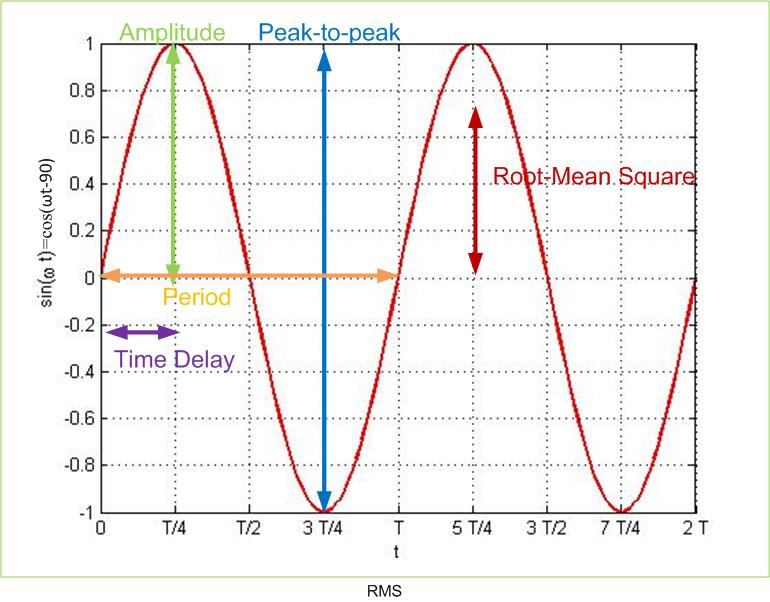
\includegraphics[scale=0.4]{../jpg/sinusoid.jpg}
\caption{Vocabulary used in describing sinusoidal signals.}
\label{sinusoid}
\end{center}
\end{figure} 


\subsection{Parameters that are read on y-axis.}

\begin{definition}
Peak amplitude is measured on the y-axis as the length from the average value of the signal (in this case zero) to the maximum value of the signal (in this case 1). For signal shown in Figure \ref{sinusoid}, the peak  amplitude has a constant value of $V_p=1$. 
\end{definition}


\begin{definition}
Instantaneous value of the sinusoidal signal varies from -1 to 1V, and depends on where on the x-axis are we observing the instantaneous value. 

Compared to the instantaneous value, the peak amplitude is allways constant and it does not vary with time. 
\end{definition}

\begin{definition}
Peak-to-peak is measured from the minimum value of the function (in this case -1) to the maximum value of the function (in this case 1).  For signal shown in Figure \ref{sinusoid}, peak-to-peak voltage has a constant value of  $V_{pp}=2$.
\end{definition}

\begin{definition}
RMS or root-mean-square is defined as $v_{rms}=\frac{1}{T} \sqrt{\int_0^T v(t)^2 dt}$. For signal shown in Figure \ref{sinusoid}, and other sinusoidal signals of this form,  $v_{rms}=\frac{V_p}{\sqrt{2}}=\frac{1}{\sqrt{2}}=0.707$. Root mean square value is important because it represents the equivalent amount of DC power.
\end{definition}


\begin{definition}
Average value $v_{ave1}=\frac{1}{T} \int_0^T v(t) dt$. For the signal shown in Figure \ref{sinusoid}, the average value is $V_{ave1}=0$ because the function has the same area under the function in the positive and negative cycle. 
\end{definition}

\subsection{Parameters that are read on the x-axis.}

\begin{definition}
Sinusoidal signals can be represented as a function of time, Figure \ref{sin}, or a function of angle, Figure \ref{sinPh}. Take a few minutes to see how the graphs are the same and how are they different.



\begin{figure}[htpb]
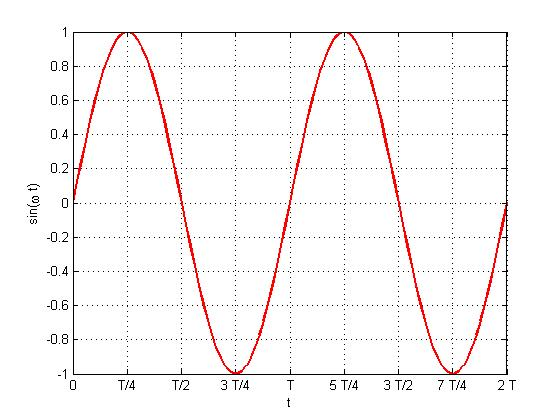
\includegraphics[scale=0.4]{../jpg/cpef1.jpg}
\caption{$sin ( \omega t)$ as a function of time.} \label{sin}
\end{figure}




\begin{figure}[htpb]
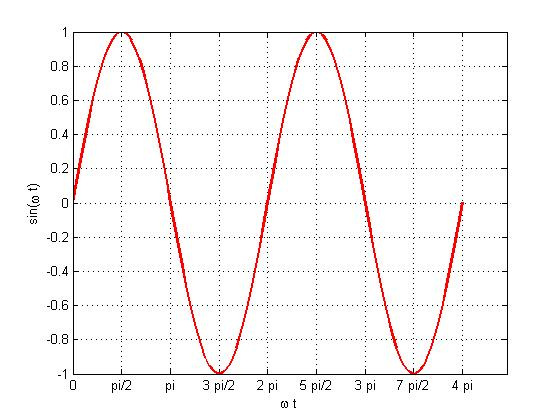
\includegraphics[scale=0.4]{../jpg/cpef3.jpg}
\caption{Sinusoidal signal as a function of angle $\omega t$.}
\label{sinPh}
\end{figure}

\end{definition}


\begin{definition}
Period, T, is measured on the x-axis as the length of one full cycle of the sinusoidal signal. For signal shown in Figure \ref{sinusoid}, this value is $period=T$. 
\end{definition}

\begin{definition}
Frequency, f,  is defined as a reciprocal value of the period T, $f=\frac{1}{T}$. It represents how fast is the signal changing in time.  In Figure \ref{sinF1F2}, sinusoidal signals of two different frequencies f are given. 

\begin{figure}[htbp]
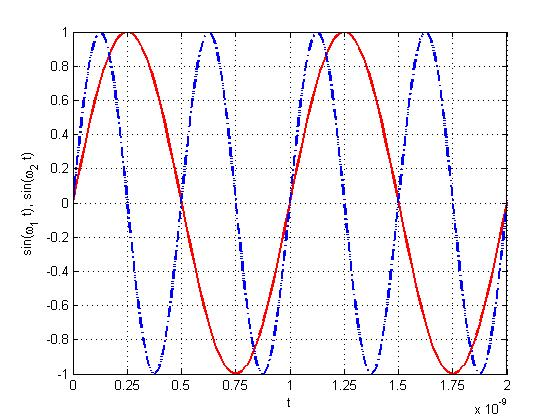
\includegraphics[scale=0.4]{../jpg/cpef6.jpg}
\caption{Sinusoidal signals of different frequencies $sin ( \omega t)$}
\label{sinF1F2}
\end{figure}

\end{definition}

\subsubsection{Phase and time-delay}


\begin{definition}
How do we recognize lagging and leading on a graph? 

In Figure \ref{timedelaysig} we observe two step functions, V(t) and V(t-T). Function V(t) step occurs at t=0, and V(t-T) step occurs at t=T. The function V(t-T) is shifted to the right, the step occurs later in time, at t=T, and is therefore lagging with respect to function V(t). 


Similarly, if the step function is given as V(t+T), then the function is shifted to the left, the step occurs earlier in time at t=-T, therefore V(t-T) is leading V(t).


\begin{figure}[htbp]
\begin{center}
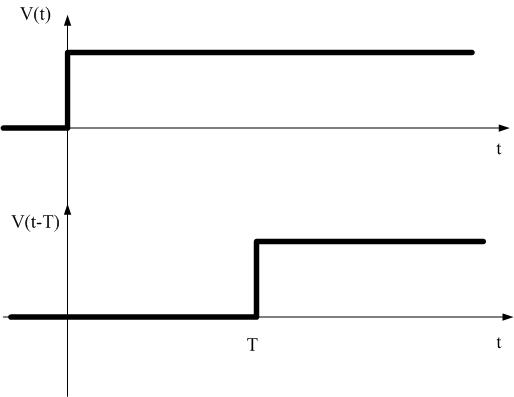
\includegraphics[scale=0.5]{../jpg/timedelayedsignal.jpg}  
%\strut\psfig{figure=generaltransmissionlinecircuit.ps,width=3cm}
\end{center}
\caption{Voltage as a function of time at the generator side z=0 (top) and the load side z=l (bottom) of the transmission line in Figure \ref{elcric}, if the switch closes at t=0 the voltage arrives at t=l/c=T at the load. These graphs can be obtained by observing the voltage on an oscilloscope at the load and at the generator side.}
\label{timedelaysig} 
 \end{figure}
\end{definition}



\begin{example}

What if we have a sinusoidal signal? We will similarly look at a specific point on the signal, for example the maximum value, and determine if it shifted left or right on the graph.

When the phase of a signal is positive as in Figure \ref{sinPlus45Ph} $ \sin (\omega t + 45^o)$, we say that the signal is leading with respect to the signal $v(t)= \sin (\omega t)$, because it is shifted to the left for $45^o$($pi/4$). The maximum of the function now occurs at t=-T, or $\omega t = -45^o$, and the new function can be written as the original sinusoidal function V(t) shifted left for a time T,  V(t+T). The phase of the signal is $45^o$, and the time-delay is T. 


\begin{figure}[htbp]
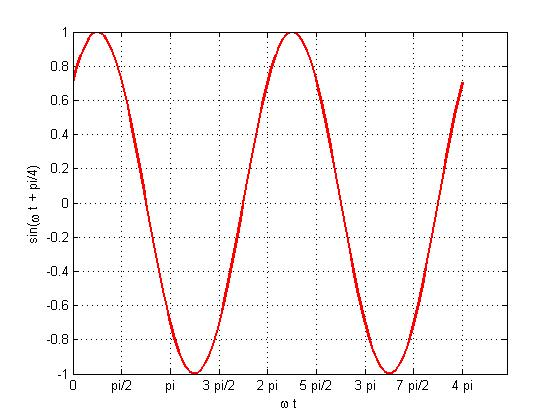
\includegraphics[scale=0.4]{../jpg/cpef5.jpg}
\caption{Sinusoidal signal as a function of angle $\omega t$ with a phase shift of $+\pi/4$}
\label{sinPlus45Ph}
\end{figure}

\end{example}



\begin{question}
Sinusoidal signal $v_1=\cos(\omega t - 25^o)$ is given. Compared to $v=\cos(\omega t)$, signal $v_1$
\begin{multipleChoice}  
\choice{Leads signal $v$}
\choice[correct]{Lags signal $v$}   
\end{multipleChoice}
\end{question}


\begin{definition}
Time delay and phase represent the lag (or lead) of one function with respect to another in time domain and frequency domain. For example, in Figure \ref{sinusoid}, function $ \cos(\omega t - 90^o)$ is time-delayed for $\tau = \frac{T}{4}$ with respect to $\cos (\omega t)$. To find the time delay for a sinusoidal signal from its phase, we look at the way to represent the phase $90^o$ in terms of the product of frequency and time. Since in the sinusoidal signal expression $\cos (\omega t + \Theta)$  phase $\Theta$ is added to $\omega t$ term, the phase has the same units as $\omega t$, and can be represented as the product of $\omega \tau = \theta$, $\tau = \frac{\theta}{\omega}$, where $\tau$ represents the time delay.
\end{definition}









\begin{figure} [htbp]
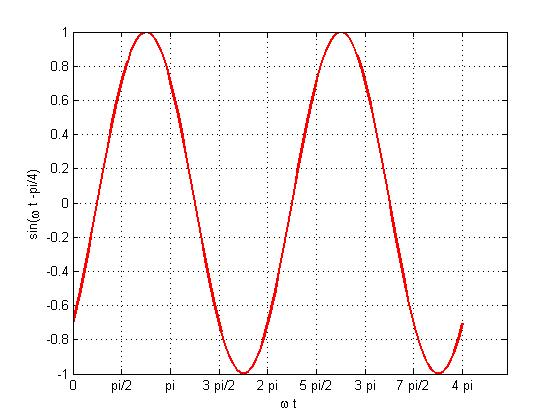
\includegraphics[scale=0.4]{../jpg/cpef4.jpg}
\caption{Sinusoidal signal as a function of angle $\omega t$ with a phase shift of $-\pi/4$}
\label{sinMinus45Ph}
\end{figure}

\begin{example}
\item When the phase of a signal is negative as in Figure \ref{sinMinus45Ph}, \ref{sinMinus45T},  $ \sin (\omega t - 45^o)$, we say that the signal is lagging with respect to the signal $ \sin (\omega t)$, because it is shifted to the right for $45^o$ ($pi/4$), or $\tau=-\frac{pi/4}{\omega} $. The lagging function's peak occurs later in time, and therefore it is lagging. The phase of the signal is $-45^o$.


\begin{figure}[htbp]
\begin{center}
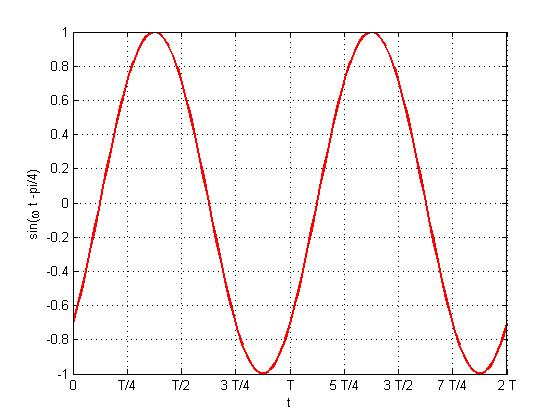
\includegraphics[scale=0.4]{../jpg/cpef2.jpg}
\caption{ Sinusoidal signal shifted for time delay $-\frac{\pi/4}{\omega}$}
\label{sinMinus45T}
\end{center}
\end{figure}



\end{example}


\begin{question}  
Calculate the time-delay in nanoseconds that you would observe on an oscilloscope if the frequency of the signal is f=0.159\,GHz and the phase shift of the signal is $\theta=10^o$. \\
$ \frac{\theta}{2*\pi*f} = \answer{10}$  ns
\end{question} 




\begin{question}  

Three signals are given in Figure below


\begin{image}
\begin{tikzpicture}
    \begin{axis}[
            xmin=-6.75,xmax=6.75,ymin=-1.5,ymax=1.5,
            axis lines=center,
            xtick={-6.28, -4.71, -3.14, -1.57, 0, 1.57, 3.142, 4.71, 6.28},
            xticklabels={$-2\pi$,$-3\pi/2$,$-\pi$, $-\pi/2$, $0$, $\pi/2$, $\pi$, $3\pi/2$, $2\pi$},
            ytick={-1,1},
            %ticks=none,
            width=6in,
            height=3in,
            unit vector ratio*=1 1 1,
            xlabel=$\theta$, ylabel=$x$,
            every axis y label/.style={at=(current axis.above origin),anchor=south},
            every axis x label/.style={at=(current axis.right of origin),anchor=west},
          ]        
          \addplot [very thick, penColor, samples=100,smooth, domain=(-6.75:6.75)] {cos(deg(x))};
        \addplot [very thick, penColor4, samples=100,smooth, domain=(-6.75:6.75)] {cos(deg(x)+90)};
         \addplot [very thick, penColor2, samples=100,smooth, domain=(-6.75:6.75)] {cos(deg(x)-90)};
                   
          \node at (axis cs:-3,-1.2) [penColor] {$\cos(\theta)$};
          \node at (axis cs:-1.72, 1.2) [penColor4] {$\cos(\theta + \pi/4)$};
        \node at (axis cs:3, 1.2) [penColor2] {$\cos(\theta - \pi/4)$};
        \end{axis}
\end{tikzpicture}
%% \caption{The function $\cos(\theta)$ takes on all values between $-1$
%%   and $1$ exactly once on the interval $[0,\pi]$. If we restrict
%%   $\cos(\theta)$ to this interval, then this restricted function has
%%   an inverse.}
%% \label{figure:cos-restricted}
%% \end{figure*}
\end{image}


Which of the following functions leads $\cos(\omega t)$?  
\begin{multipleChoice}  
\choice[correct]{The green signal.}  
\choice{The red signal.}  
\choice{The blue signal.}  
\end{multipleChoice}  
\end{question}

\begin{example}

Lagging and leading is often used in circuits to describe signals.

Let's look at a circuit in Figure \ref{elcric} where the generator and the load are connected with a cable, just as in your circuits lab. The cable is overemphasised in this figure, compared to figures in your circuits lab, where the cable is usually ignored. 


Let's assume that the switch closes, and the generator produces a step function at time t=0, as shown in Figure  \ref{timedelaysig}. Because the electrical signals propagate with the speed of light, the signal needs T sec to appear at the load, after the switch closes. Figure \ref{delayedsig} shows the step signal as it traveles on the transmission line at different times t=0, t=T/4, t=T/2 and t=T.



 How much time T does it take for this signal to go from AA' end to BB' end? 
Since electromagnetic waves propagate with the constant speed, the speed of light, time that  the signal needs to go from the generator to  the load  depends  on the length of the transmission line. If the transmission line is $l$, then the delay between the generator and the load will be  $T=\frac{l}{c}$, where $c=3\times 10^8$. If the signal at the generator AA' is $v_g(t)=$v(t), then the signal at the load end is $v_l(t)=$v(t-T). 



\begin{figure}[htbp]
\begin{center}
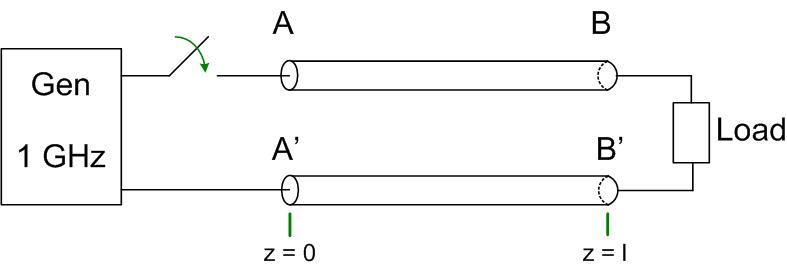
\includegraphics[scale=0.5]{../jpg/generaltransmissionlinecircuit1.jpg}
%\strut\psfig{figure=generaltransmissionlinecircuit.ps,width=3cm} \\
\end{center}
\caption{Electronic Circuit with an emphasis on cables that connect the generator and the load.}
\label{elcric}
\end{figure}




\begin{figure}[htbp]
\begin{center}
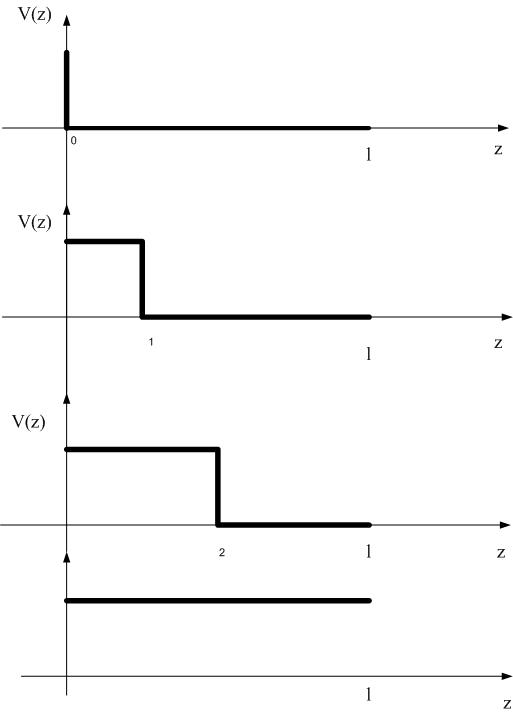
\includegraphics[scale=0.5]{../jpg/timedelayedsignaltl.jpg}
%\strut\psfig{figure=generaltransmissionlinecircuit.ps,width=3cm} \\
\end{center}
\caption{Voltage along the transmission line in Figure \ref{elcric}, for four different time intervals t=0, switch closes, t=T/4, t=T/2 and t=T. It is assumed that the length of the transmission line is equal to l=T/c.Note that the horizontal axis is the distance z from the generator to the cable, not time. }
\label{delayedsig}
\end{figure}

\end{example}



\begin{example}
Application of sinusoidal signals to engineering design. When do we have to use transmission-line theory? The answer to this question depends on the delay (or phase shift) that the line introduces.

If we have a sinusoidal generator at the beginning of the transmission line, instead of the step signal, what would the signal look like when it arrives at the load?

The signal at the generator is 

\begin{eqnarray}
v_{AA^`}(t)=A cos(\omega t)
\end{eqnarray}

At the other end the transmission line the signal is delayed


\begin{eqnarray}
v_{BB^`}(t)=v_{AA^`}(t-T) \\
v_{BB^`}(t)=v_{AA^`}(t-\frac{l}{c}) \\
v_{BB^`}(t)=A cos(\omega (t - \frac{l}{c}))  \\
v_{BB^`}(t)=A cos(\omega t - \omega \frac{l}{c}) \\
v_{BB^`}(t)=A cos(\omega t -  \frac{\omega }{c} l) 
\end{eqnarray}

Since we know that angular frequency is  $\omega = 2 \pi f$


\begin{eqnarray}
v_{BB^`}(t)=A cos(\omega t -  \frac{ 2 \pi f }{c} l)
\end{eqnarray}

The quantity $\frac{c}{f}$ is called the wavelength $\lambda$. 

\begin{eqnarray}
v_{BB^`}(t)=A \, cos(\omega t -  \frac{ 2 \pi }{\lambda} l) \label{tllength1}
\end{eqnarray}

The quantity $ \frac{ 2 \pi }{\lambda} $ is the propagation constant $\beta$


Finally the expression for the voltage at BB end is


\begin{eqnarray}
v_{BB^`}(t)=A \, cos(\omega t - \beta l) \\
v_{BB^`}(t)=A \, cos(\omega t - \Psi)
\end{eqnarray}

We see that at BB' the signal will experience a delay  (a.k.a. phase shift).
We will later show that the solution of the wave equation is the equation above. We will derive this equation  again later from the Telegrapher's
equations.
Now let's see how the length of the line $l$ affects the voltage at the
end BB'. Look at Equation \ref{tllength1}.
The signal will experience a phase shift of $2\pi \frac{l}{\lambda}$. If this phase shift is small, there will not be much difference between
the phase of the signal at the generator and at the load. This means that we don't have to use transmission line theory to account for the effects of the line.
If the phase shift is significant, then we do have to use the transmission line theory. Let's look at some numbers in the  following example.

\begin{enumerate}
\item If $\frac{l}{\lambda} < 0.01$ then the angle $2 \pi
\frac{l}{\lambda}$ is of the order of 0.0314 rad or about 2$^0$. In this case, the
phase is obviosly something that we don't have to worry about. When
the length of the transmission line is much smaller than $\lambda$, $l<<\frac{\lambda}{100}$
the wave propagation on the line can be ingnored.
\item If  $\frac{l}{\lambda} > 0.01$, say  $\frac{l}{\lambda} =0.1$,
then the phase is 20$^0$, which is a significant phase shift. In this
case it may be necessary to account fro transmission line effects.
\end{enumerate}

\end{example}








%\begin{image}
%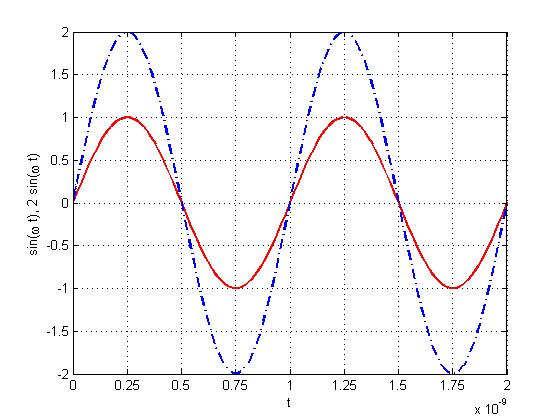
\includegraphics[scale=0.4]{jpg/cpef7.jpg}
%\caption{Sinusoidal signals of different amplitudes $sin ( \omega t)$}\label{sinA1A2}
%\end{image}




%\begin{image}
%\begin{tikzpicture}
%    \begin{axis}[
%            xmin=-6.75,xmax=6.75,ymin=-1.5,ymax=1.5,
%            axis lines=center,
%            xtick={-6.28, -4.71, -3.14, -1.57, 0, 1.57, 3.142, 4.71, 6.28},
%            xticklabels={$-2\pi$,$-3\pi/2$,$-\pi$, $-\pi/2$, $0$, $\pi/2$, $\pi$, $3\pi/2$, $2\pi$},
%            ytick={-1,1},
%            %ticks=none,
%            width=6in,
%            height=3in,
%            unit vector ratio*=1 1 1,
%            xlabel=$\theta$, ylabel=$x$,
%            every axis y label/.style={at=(current axis.above origin),anchor=south},
%            every axis x label/.style={at=(current axis.right of origin),anchor=west},
%          ]        
%          \addplot [very thick, penColor, samples=100,smooth, domain=(-6.75:6.75)] {cos(deg(x))};
%        \addplot [very thick, penColor4, samples=100,smooth, domain=(-6.75:6.75)] {cos(deg(x)+90)};
%         \addplot [very thick, penColor2, samples=100,smooth, domain=(-6.75:6.75)] {cos(deg(x)-90)};
%                   
%          \node at (axis cs:-3,-1.2) [penColor] {$\cos(\theta)$};
%          \node at (axis cs:-1.72, 1.2) [penColor4] {$\cos(\theta + \pi/4)$};
%        \node at (axis cs:3, 1.2) [penColor2] {$\cos(\theta - \pi/4)$};
%        \end{axis}
%\end{tikzpicture}
%% \caption{The function $\cos(\theta)$ takes on all values between $-1$
%%   and $1$ exactly once on the interval $[0,\pi]$. If we restrict
%%   $\cos(\theta)$ to this interval, then this restricted function has
%%   an inverse.}
%% \label{figure:cos-restricted}
%% \end{figure*}
%\end{image}

  

\end{document}



                                                                   



                                       




                                    















